% generated by scripts/pkl_to_latex.py
% source PKL : thermal_v1_L8_Ne8_U10_t0p1_mode-uniform_tpall_t2all_tperpall_nmin2_solver-gcg_full_restarts4_iter200_kmax4_tol1em09_cut10_adaptive1_step5_clusteravg1_T0to5_N40-205b87919d2f_knone_diag0.pkl
% scan type  : Tscan
% state      : gs
% requires   : \usepackage{pgfplots} \pgfplotsset{compat=1.18}
% colours match the matplotlib PDF (tab10 cycle)
\definecolor{gmeC0}{HTML}{1F77B4}
\definecolor{gmeC1}{HTML}{FF7F0E}
\definecolor{gmeC2}{HTML}{2CA02C}
\definecolor{gmeC3}{HTML}{D62728}
\definecolor{gmeC4}{HTML}{9467BD}
\definecolor{gmeC5}{HTML}{8C564B}
\definecolor{gmeC6}{HTML}{E377C2}
\definecolor{gmeC7}{HTML}{17BECF}

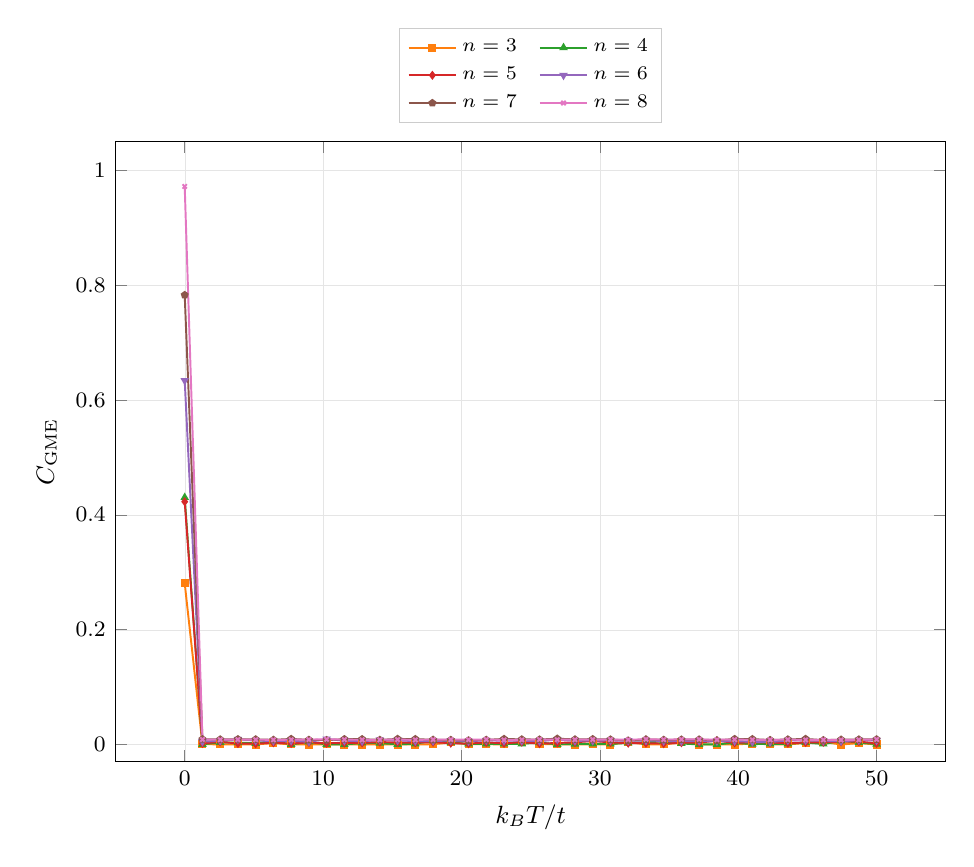
\begin{tikzpicture}
  \begin{axis}[
    width=\columnwidth,
    height=0.78\columnwidth,
    xlabel={$k_B T/t$},
    ylabel={$C_{\mathrm{GME}}$},
    grid=both,
    grid style={line width=.1pt, draw=gray!20},
    tick label style={font=\footnotesize\rmfamily, /pgf/number format/fixed},
    label style={font=\small\rmfamily},
    scaled ticks=false,
    legend style={font=\scriptsize\rmfamily, draw=gray!40, at={(0.5,1.03)}, anchor=south, /tikz/every even column/.append style={column sep=6pt}},
    legend cell align={left},
    legend columns=2,
    ymin=-0.03,
    ymax=1.05,
  ]
    \addplot[color=gmeC1, mark=square*, mark size=1.1pt, line width=0.7pt] coordinates {
        (0,0.280758) (1.282051,0.00078) (2.564103,0.000125) (3.846154,0.000123)
        (5.128205,0.000035) (6.410256,0.002635) (7.692308,0.000065) (8.974359,0)
        (10.25641,0.000311) (11.538462,0.000016) (12.820513,0.000007) (14.102564,0.000016)
        (15.384615,0.000001) (16.666667,0.000034) (17.948718,0.000526) (19.230769,0.003581)
        (20.512821,0.000422) (21.794872,0.000513) (23.076923,0.000239) (24.358974,0.00514)
        (25.641026,0.001207) (26.923077,0.000072) (28.205128,0.000034) (29.487179,0.000114)
        (30.769231,0.000002) (32.051282,0.004229) (33.333333,0.00028) (34.615385,0.000102)
        (35.897436,0.003541) (37.179487,0.000035) (38.461538,0.000025) (39.74359,0.000016)
        (41.025641,0.001783) (42.307692,0.000317) (43.589744,0.000116) (44.871795,0.002703)
        (46.153846,0.004606) (47.435897,0.000013) (48.717949,0.002487) (50,0.000029)
    };
    \addlegendentry{$n=3$}
    \addplot[color=gmeC2, mark=triangle*, mark size=1.1pt, line width=0.7pt] coordinates {
        (0,0.430247) (1.282051,0.000366) (2.564103,0.003786) (3.846154,0.003257)
        (5.128205,0.002155) (6.410256,0.005719) (7.692308,0.000329) (8.974359,0.004451)
        (10.25641,0.00033) (11.538462,0.000038) (12.820513,0.002719) (14.102564,0.002533)
        (15.384615,0.00031) (16.666667,0.001309) (17.948718,0.006773) (19.230769,0.003419)
        (20.512821,0.001102) (21.794872,0.001043) (23.076923,0.001165) (24.358974,0.001265)
        (25.641026,0.00348) (26.923077,0.000347) (28.205128,0.000718) (29.487179,0.001285)
        (30.769231,0.001039) (32.051282,0.002752) (33.333333,0.003868) (34.615385,0.005418)
        (35.897436,0.001851) (37.179487,0.00006) (38.461538,0.000156) (39.74359,0.003186)
        (41.025641,0.000685) (42.307692,0.001195) (43.589744,0.001161) (44.871795,0.003521)
        (46.153846,0.000898) (47.435897,0.006405) (48.717949,0.003495) (50,0.000715)
    };
    \addlegendentry{$n=4$}
    \addplot[color=gmeC3, mark=diamond*, mark size=1.1pt, line width=0.7pt] coordinates {
        (0,0.422854) (1.282051,0.00183) (2.564103,0.00479) (3.846154,0.001682)
        (5.128205,0.001352) (6.410256,0.003053) (7.692308,0.001739) (8.974359,0.003624)
        (10.25641,0.002114) (11.538462,0.002761) (12.820513,0.00289) (14.102564,0.004266)
        (15.384615,0.003516) (16.666667,0.00323) (17.948718,0.00401) (19.230769,0.00233)
        (20.512821,0.001496) (21.794872,0.003748) (23.076923,0.002038) (24.358974,0.004164)
        (25.641026,0.001552) (26.923077,0.002678) (28.205128,0.003827) (29.487179,0.006119)
        (30.769231,0.003683) (32.051282,0.002337) (33.333333,0.00236) (34.615385,0.001548)
        (35.897436,0.003096) (37.179487,0.003326) (38.461538,0.006618) (39.74359,0.002956)
        (41.025641,0.003971) (42.307692,0.003443) (43.589744,0.002265) (44.871795,0.003499)
        (46.153846,0.003887) (47.435897,0.00485) (48.717949,0.005102) (50,0.002061)
    };
    \addlegendentry{$n=5$}
    \addplot[color=gmeC4, mark=triangle*, mark size=1.1pt, mark options={rotate=180}, line width=0.7pt] coordinates {
        (0,0.633885) (1.282051,0.004941) (2.564103,0.006532) (3.846154,0.008907)
        (5.128205,0.006761) (6.410256,0.006134) (7.692308,0.006603) (8.974359,0.004613)
        (10.25641,0.009594) (11.538462,0.006596) (12.820513,0.005729) (14.102564,0.007945)
        (15.384615,0.007097) (16.666667,0.006049) (17.948718,0.006057) (19.230769,0.006897)
        (20.512821,0.005548) (21.794872,0.007423) (23.076923,0.00653) (24.358974,0.006554)
        (25.641026,0.005855) (26.923077,0.008665) (28.205128,0.006364) (29.487179,0.006713)
        (30.769231,0.00705) (32.051282,0.00662) (33.333333,0.007017) (34.615385,0.006123)
        (35.897436,0.005925) (37.179487,0.006096) (38.461538,0.005863) (39.74359,0.006014)
        (41.025641,0.004587) (42.307692,0.004255) (43.589744,0.007228) (44.871795,0.007215)
        (46.153846,0.006239) (47.435897,0.005529) (48.717949,0.00758) (50,0.007137)
    };
    \addlegendentry{$n=6$}
    \addplot[color=gmeC5, mark=pentagon*, mark size=1.1pt, line width=0.7pt] coordinates {
        (0,0.782789) (1.282051,0.009165) (2.564103,0.008794) (3.846154,0.00923)
        (5.128205,0.008937) (6.410256,0.00811) (7.692308,0.009683) (8.974359,0.008172)
        (10.25641,0.007673) (11.538462,0.00931) (12.820513,0.009284) (14.102564,0.008058)
        (15.384615,0.009752) (16.666667,0.009455) (17.948718,0.00816) (19.230769,0.007932)
        (20.512821,0.007153) (21.794872,0.008098) (23.076923,0.009674) (24.358974,0.00892)
        (25.641026,0.008654) (26.923077,0.010159) (28.205128,0.008847) (29.487179,0.009387)
        (30.769231,0.008701) (32.051282,0.00693) (33.333333,0.009005) (34.615385,0.008098)
        (35.897436,0.008542) (37.179487,0.008722) (38.461538,0.00726) (39.74359,0.009614)
        (41.025641,0.00938) (42.307692,0.007835) (43.589744,0.008781) (44.871795,0.00973)
        (46.153846,0.007556) (47.435897,0.00843) (48.717949,0.00873) (50,0.008972)
    };
    \addlegendentry{$n=7$}
    \addplot[color=gmeC6, mark=x, mark size=1.1pt, line width=0.7pt] coordinates {
        (0,0.971886) (1.282051,0.008817) (2.564103,0.008317) (3.846154,0.008509)
        (5.128205,0.008348) (6.410256,0.008143) (7.692308,0.008294) (8.974359,0.008595)
        (10.25641,0.009128) (11.538462,0.008559) (12.820513,0.008132) (14.102564,0.00819)
        (15.384615,0.008632) (16.666667,0.008008) (17.948718,0.008545) (19.230769,0.008538)
        (20.512821,0.008401) (21.794872,0.008731) (23.076923,0.007887) (24.358974,0.008065)
        (25.641026,0.008658) (26.923077,0.008466) (28.205128,0.008409) (29.487179,0.008632)
        (30.769231,0.008598) (32.051282,0.008438) (33.333333,0.009076) (34.615385,0.008608)
        (35.897436,0.008926) (37.179487,0.008972) (38.461538,0.008306) (39.74359,0.008633)
        (41.025641,0.008082) (42.307692,0.00803) (43.589744,0.008539) (44.871795,0.007941)
        (46.153846,0.008077) (47.435897,0.007891) (48.717949,0.008146) (50,0.008935)
    };
    \addlegendentry{$n=8$}
  \end{axis}
\end{tikzpicture}
